\documentclass[border=7pt] {standalone}
\usepackage{tikz}
\usepackage{amsmath}
\usepackage{amsfonts}
\usepackage{amssymb} 
\definecolor{mycolor}{RGB}{30,51,76}
\definecolor{hi}{RGB}{66, 134, 244}

\begin{document}


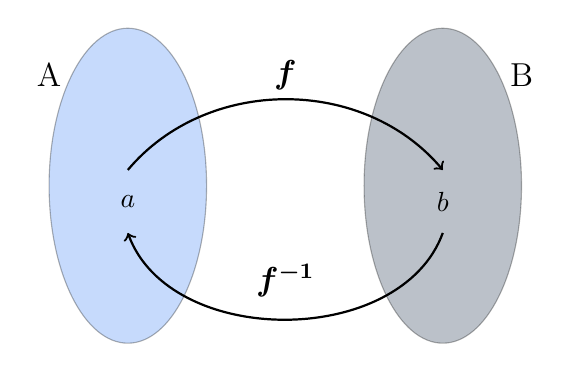
\begin{tikzpicture}

\draw (1,2)[fill=hi, opacity=0.3] ellipse (1cm and 2cm);
\draw (5,2)[fill=mycolor, opacity=0.3] ellipse (1cm and 2cm);
\node (c) at (0 ,3.4) {\large A};
\node (c) at (6 ,3.4) {\large B};
\node (c) at ( 3,3.4) {\large $\boldsymbol{f}$};
\draw[->, thick] (1,2.2) to [out=50 , in = 130] (5,2.2);
\node (c) at ( 3,0.8) {\large $\boldsymbol{f^{-1}}$};
\node (c) at (1,1.8) {$a$};
\node (c) at (5,1.8) {$b$};
\draw[<-, thick] (1,1.4) to [out=290 , in = 250] (5,1.4);

\end{tikzpicture}
\end{document}
